\documentclass[11pt, oneside]{article}   	% use "amsart" instead of "article" for AMSLaTeX format
\usepackage{geometry}                		% See geometry.pdf to learn the layout options. There are lots.
\geometry{letterpaper}                   		% ... or a4paper or a5paper or ... 
%\geometry{landscape}                		% Activate for rotated page geometry
%\usepackage[parfill]{parskip}    		% Activate to begin paragraphs with an empty line rather than an indent
\usepackage{graphicx}				% Use pdf, png, jpg, or eps§ with pdflatex; use eps in DVI mode
\usepackage{caption}
\usepackage{subcaption}								% TeX will automatically convert eps --> pdf in pdflatex	
\usepackage{amssymb}
\usepackage{eqnarray,amsmath}
\usepackage{ marvosym}

\usepackage{wesu}
\usepackage[T1]{fontenc}

\usepackage{calligra}
\usepackage[T1]{fontenc}

%SetFonts

%SetFonts




					% Activate to display a given date or no date

\begin{document}
\baselineskip=20pt

\title{Capstone Project of Machine Learning Engineer Nanodegree: Plot and Navigate a Virtual Maze}
\author{\wesu Yi-Yuan Chiang}
\maketitle
\section{Definition}
There are three subsections in this section. They are: {\it Project Overview}, {\it Problem Statement}, and {\it Metrics}.

\subsection{Project Overview}
The purpose of this project is to design a virtual robot to navigate a given maze. The task of the robot is to plot a path from a corner of the maze to the center. Two runs are allowed. In the first run, the robot has to find the goal and the best path from corner to center. In the second run, the robot attempts to reach the center in the fastest time possible, using what it has learned in the first run. This rule is inspired from the APEC Micromouse Contest {\cite {apec}}.
\subsection{Problem Statement}
As mentioned in the previous section, two runs are allowed for the robot. In the first run, the robot is allowed to freely roam the maze to build a map of the maze. It must enter the goal room at some point during its exploration, but is free to continue exploring the maze after finding the goal. After entering the goal room, the robot may choose to end its exploration at any time. The robot is then moved back to the starting position and orientation for its second run. Its objective now is to go from the start position to the goal room in the fastest time possible.
\subsection{Metrics}
The robot's score for the maze is equal to the number of time steps required to execute the second run, plus one thirtieth the number of time steps required to execute the first run. A maximum of one thousand time steps is allotted to complete both runs for a single maze.
%%%%%%%%%%%%%%%%%%%%%%%%%%%%%%%%%%%%%%%%%%%%%%%%%%%%%%%%%%%%%%%%%%%%%%%%%%%%%%%%%%%%
\section{Analysis}
There are three subsections in this section. They are: {\it Data Exploration and Visualization}, {\it Algorithms and Techniques}, and {\it Benchmark}.
\subsection{Data Exploration and Visualization}
The given mazes are specified and coded in the files with text format. On the first line of the text file is a number, $n$, describing the number of squares on each dimension of the maze. 

On the following $n$ lines are $n$ comma-delimited four-bit coding numbers describing which edges of the square are open to movement. The coding method is described as below. Each number represents a four-bit number that has a bit value of $0$ if an edge is closed (walled) and $1$ if an edge is open (no wall); the $1$s register corresponds with the upwards-facing side, the $2$s register the right side, the $4$s register the bottom side, and the $8$s register the left side.

Figure {\ref {fig:example}} is a portion of an example of four-bit coding maze, in the bottom left corner, the number 1 means the upper edge of this square is open, 6 means both the right edge and the bottom edge are open.

\begin{figure}[htbp] %  figure placement: here, top, bottom, or page
   \centering
   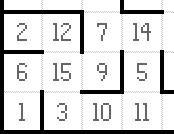
\includegraphics[width=7cm]{example.png} 
   \caption{A portion of an example of four-bit coding maze.}
   \label{fig:example} 
\end{figure}

From this coding method, we are easily to translate the given four-bit coding maze into human understandable mazes specified by walls. Figure {\ref {fig:four-bit-Maze01}} is the four-bit coding edition of Maze01; and Figure {\ref {fig:Maze01}} is the normal one.

\begin{figure}
\centering
\begin{subfigure}{7cm}
  \centering
  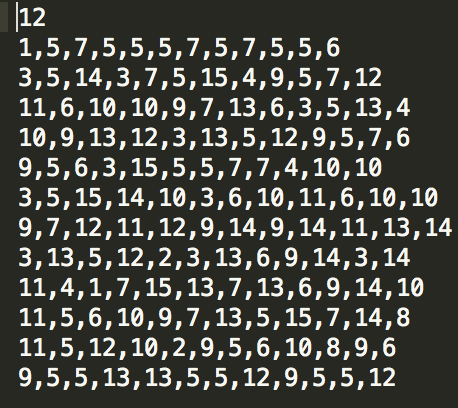
\includegraphics[width=6cm]{coded_maze01.png}
  \caption{Four-bit coding edition of Maze01. (The given format)}
  \label{fig:four-bit-Maze01}
\end{subfigure}%
\begin{subfigure}{7cm}
  \centering
  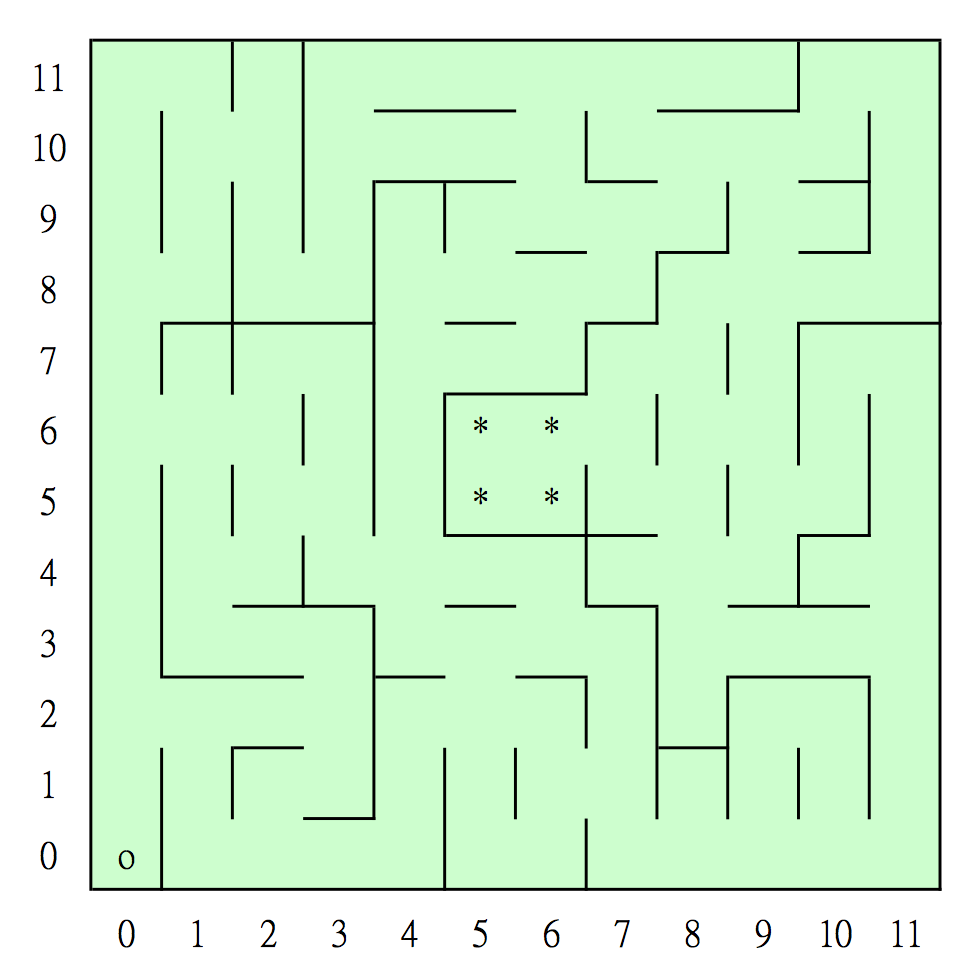
\includegraphics[width=6cm]{maze-01.png}
  \caption{Normal edition of Maze01. The start is labeled as `o' and the goal is labels as `*'.}
  \label{fig:Maze01}
\end{subfigure}
\caption{The four-bit coding representation and the normal wall representation of Maze01.}
\label{fig:test}
\end{figure}

As for robot, it has three obstacle sensors, mounted on the front of the robot, its right side, and its left side. Obstacle sensors detect the number of open squares in the direction of the sensor; for example, in its starting position, the robot's left and right sensors will state that there are no open squares in those directions and at least one square towards its front. On each time step of the simulation, the robot may choose to rotate clockwise or counterclockwise ninety degrees, then move forwards or backwards a distance of up to three units. It is assumed that the robot's turning and movement is perfect. If the robot tries to move into a wall, the robot stays where it is. After movement, one time step has passed, and the sensors return readings for the open squares in the robot's new location and/or orientation to start the next time unit.

After understand the sensing method of robot, let's take a look at maze01 more detail. The start location is $(0,0)$, and the goal is a square with four positions, they are $(5,5)$, $(5,6)$, $(6,5)$, $(6,6)$. When navigating such a maze, a robot may encounters at least two kinds of hazards. I named them as: {\it dead-end hazard} and {\it loop hazard}. When a robot encounters a dead-end hazard, it has no way for any direction except moves backwards. For example, when the robot get into the position $(1,7)$, $(4,9)$, $(8,1)$, or $(10,9)$, it encounters a dead-end hazard. The other hazard is loop hazard, which is caused by isolated walls. For example, the right-hand-side wall of position $(0,9)$ and $(0,10)$ may causes loop hazard. Our robots should avoid these hazards in the second run.

There are many paths for a robot to reach the goal. I just list three of them as shown in Figure \ref{fig:path-1}, \ref{fig:path-2}, \ref{fig:path-3}. Because the robot can move up to three units, the moving steps can be reduced. When the steps of a path are reduced, I call this path as an optimized path (Figure \ref{fig:path-1-optimized}, \ref{fig:path-2-optimized}, \ref{fig:path-3-optimized}).

\begin{figure}
\centering
\begin{subfigure}{7cm}
  \centering
  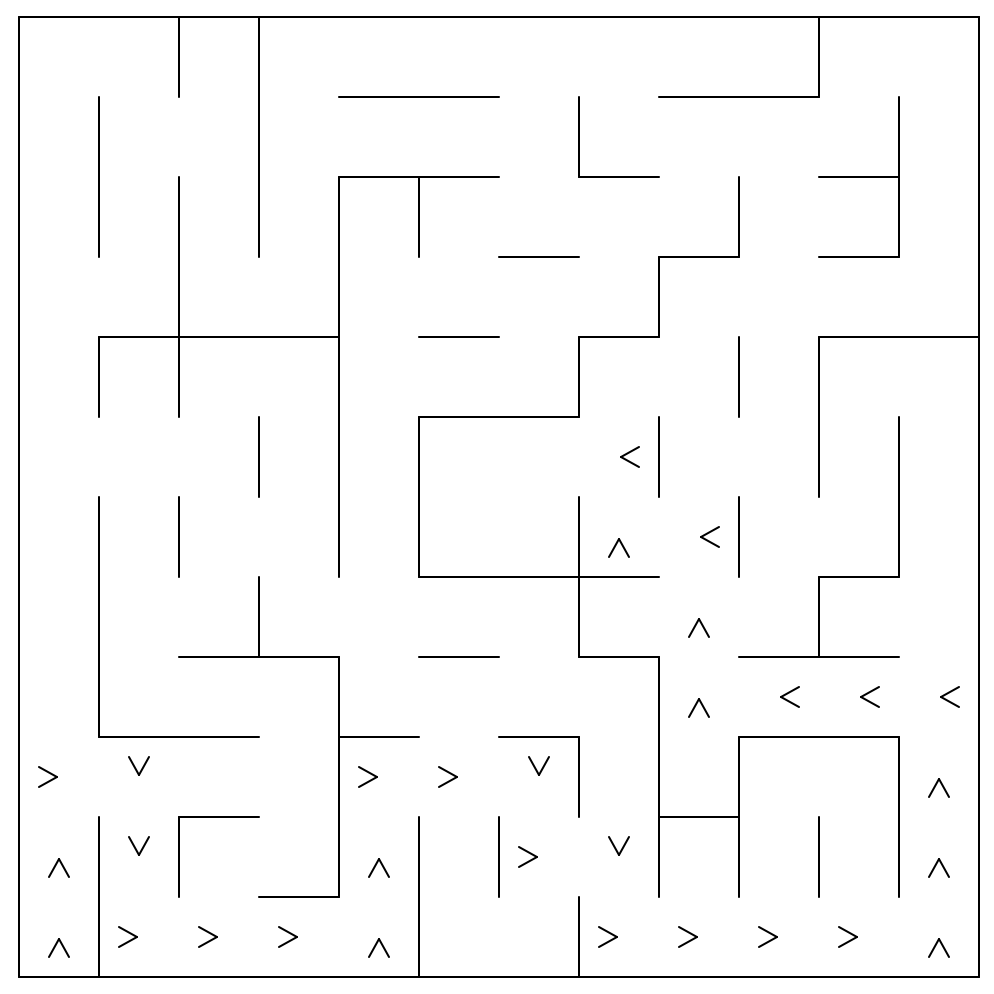
\includegraphics[width=6cm]{maze-01-1st.png}
  \caption{Maze01: path-1 (30 steps)}
  \label{fig:path-1}
\end{subfigure}%
\begin{subfigure}{7cm}
  \centering
  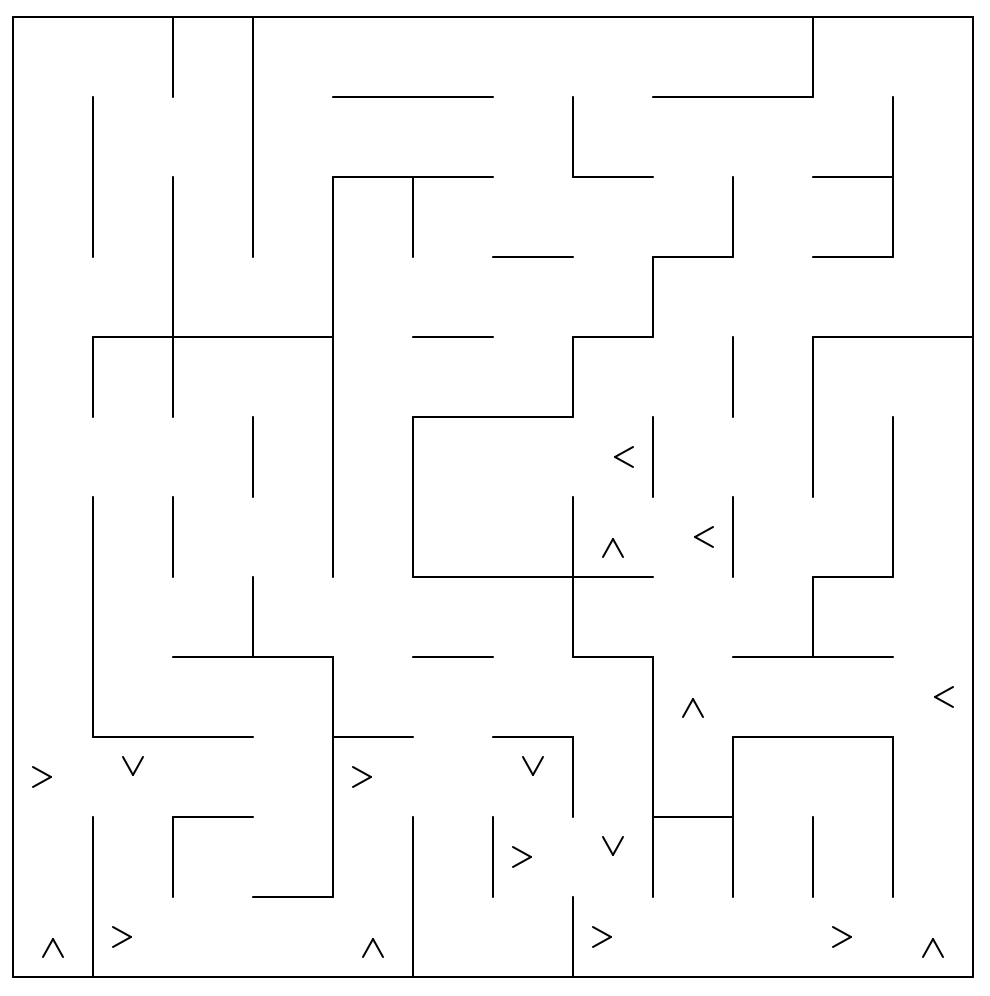
\includegraphics[width=6cm]{maze-01-1st-star.png}
  \caption{Maze01: path-1 optimized (17 steps)}
  \label{fig:path-1-optimized}
\end{subfigure}

\begin{subfigure}{7cm}
  \centering
  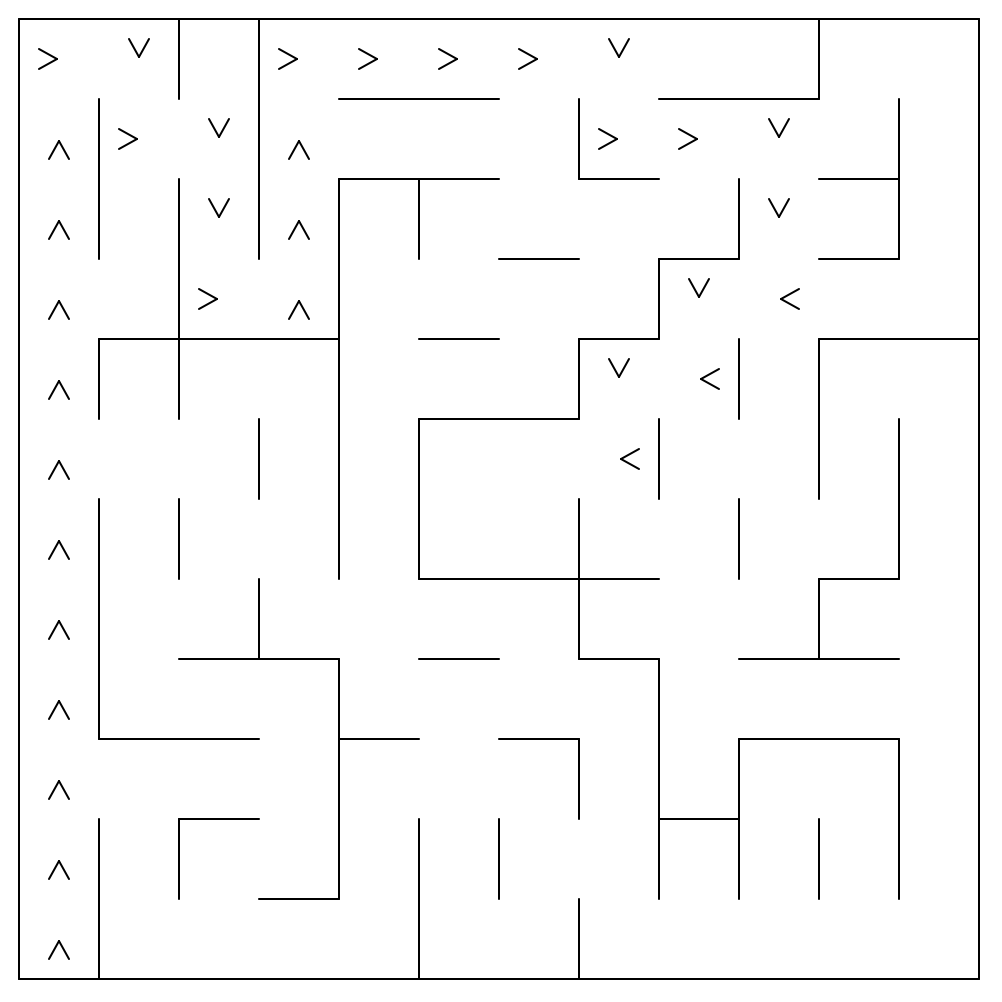
\includegraphics[width=6cm]{maze-01-2nd.png}
  \caption{Maze01: path-2 (34 steps)}
  \label{fig:path-2}
\end{subfigure}
\begin{subfigure}{7cm}
  \centering
  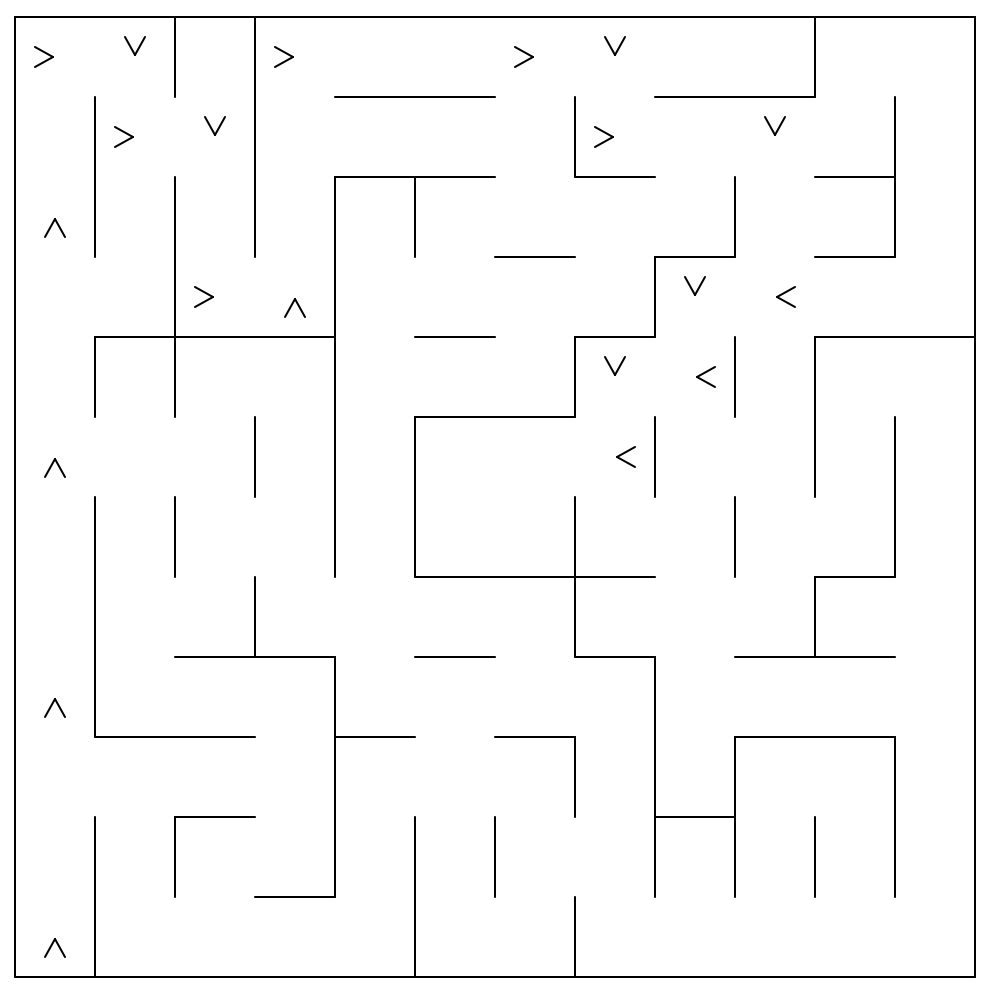
\includegraphics[width=6cm]{maze-01-2nd-star.png}
  \caption{Maze01: path-2 optimized (20 steps)}
  \label{fig:path-2-optimized}
\end{subfigure}
\begin{subfigure}{7cm}
  \centering
  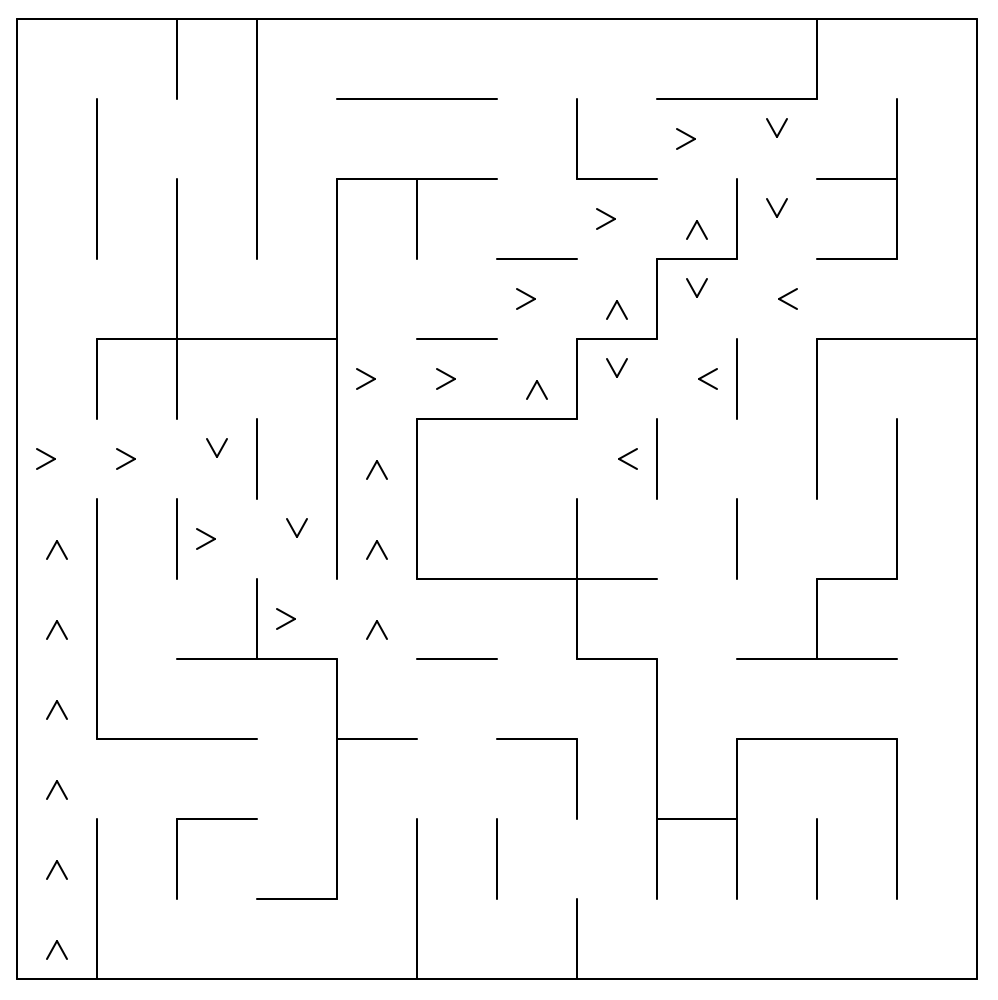
\includegraphics[width=6cm]{maze-01-3rd.png}
  \caption{Maze01: path-3 (30 steps)}
  \label{fig:path-3}
\end{subfigure}
\begin{subfigure}{7cm}
  \centering
  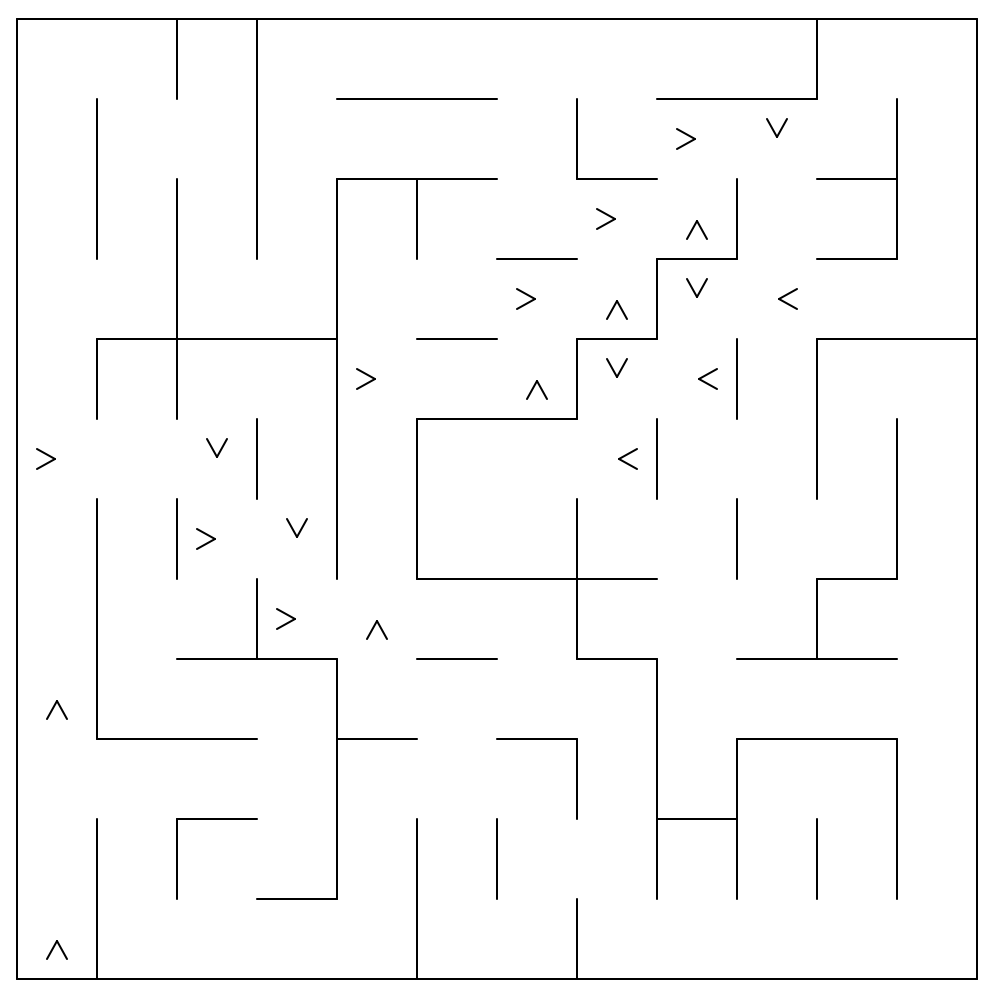
\includegraphics[width=6cm]{maze-01-3rd-star.png}
  \caption{Maze01: path-3 optimized (21 steps)}
  \label{fig:path-3-optimized}
\end{subfigure}
\caption{Example Paths of Maze01}
\label{fig:test}
\end{figure} 

The shortest path of maze01 is path-1 (Figure \ref{fig:path-1}); it takes 30 steps. After optimization, only 17 steps are required (Figure \ref{fig:path-1-optimized}).


\subsection{Algorithms and Techniques}
A robot finding a path from start to goal could be viewed as a search problem \cite{Russell-Norvig}. There are many search algorithms could be used to solve a robot path-planning problem, including {\it best-first search} (BFS), {\it uniform cost search} (UCS), {\it depth-first search} (DFS), and {\it depth-limited search} (DLS), etc \cite{G5AIAI}. These algorithms belong to {\it blind searches}, because during the search procedure, there is no additional information obtained. On the other hand, some kind of search algorithms called {\it heuristic searches}, because during the search procedure, there are additional information could be obtained. A well-known heuristic search algorithm is the A-star search \cite{Nilsson}, which will be used in this project. Except A-star search algorithm, DFS will also be implemented for the purpose of benchmarking.

A DFS could be implemented as a recursive or a non-recursive procedure. I used the non-recursive one. Notably, a maze could be viewed as a graph; all positions within the maze are interpreted as vertices or nodes of the graph. Besides, for any position, its {\it adjacent vertices} are the positions that can be arrived for a robot within one step. {\it Adjacent edges} of a node link the node and its adjacent vertices. The following is the pseudo code of DFS \cite{wikidfs}.

\begin{verbatim}
1  procedure DFS-iterative(G,v):
2      let S be a stack
3      S.push(v)
4      while S is not empty
5          v = S.pop()
6          if v is not labeled as discovered:
7              label v as discovered
8              for all edges from v to w in G.adjacentEdges(v) do
9                  S.push(w)
\end{verbatim}

As for A-star search, the following is the pseudo code \cite{Eranki}.


\begin{verbatim}

1   initialize the open list
2   initialize the closed list
3   put the starting node on the open list (you can leave its f at zero)

4   while the open list is not empty
5       find the node with the least f on the open list, call it "q"
6       pop q off the open list
7       generate q's 8 successors and set their parents to q
8       for each successor
9         if successor is the goal, stop the search
10           successor.g = q.g + distance between successor and q
11           successor.h = distance from goal to successor
12           successor.f = successor.g + successor.h

13           if a node with the same position as successor is in the OPEN list \
14               which has a lower f than successor, skip this successor
15           if a node with the same position as successor is in the CLOSED list \ 
16               which has a lower f than successor, skip this successor
17           otherwise, add the node to the open list
18        end
19        push q on the closed list
20  end


\end{verbatim}







\subsection{Benchmark}
In this subsection, I will discuss what is a reasonable benchmark score I feel. I will use the three examples stated in Section 2.1 to demonstrate what the optimal scores they could be along with the reasonable score range they perhaps will be.

As mentioned in Section 1.3, the robot's score for the maze is equal to the number of time steps required to execute the second run, plus one thirtieth the number of time steps required to execute the first run. Therefore, the scores for the paths stated in Section 2.1 should be as shown in the Table \ref{Benchmark}.

\begin{table}[htp]
\caption{The scores of path-1, path-2, and path-3.}
\begin{center}
\begin{tabular}{ rrrr } 
\hline
 & Best scores & Reasonable scores \\
\hline
path-1 & $18$    & $22 \sim 27$ \\ 
path-2 & $21.13$ & $25.67 \sim 31.33$ \\ 
path-3 & $22$    & $26 \sim 31$ \\ 
\hline
\end{tabular}
\end{center}
\label{Benchmark}
\end{table}%





%%%%%%%%%%%%%%%%%%%%%%%%%%%%%%%%%%%%%%%%%%%%%%%%%%%%%%%%%%%%%%%%%%%%%%%%%%%%%%%%%%%
\section{Methodology}
In this section, there are three subsections; they are: {\it Data Preprocessing}, {\it Implementation}, and {\it Refinement}. 
\subsection{Data Preprocessing}
Because the sensor specification and environment designs are provided, there is no data preprocessing needed in this project.
\subsection{Implementation}
The python scripts along with test mazes for this project includes the following files:
\begin{itemize}
\item robot.py: This script establishes the robot class. This is the only script I have modified.
\item maze.py: The provided script contains functions for constructing the maze and for checking for walls upon robot movement or sensing.
\item tester.py: The provided script runs to test the robot's ability to navigate mazes.
\item showmaze.py: The provided script is used to create a visual demonstration of what a maze looks like.
\item test\_maze\_01.txt $\sim$ test\_maze\_03.txt: The three provided sample files specify mazes upon which to test my robot.
\item test\_maze\_04.txt: The 12x12 maze which is designed by myself for testing the robustness of my robot.
\end{itemize}

In order to understand the architecture of the robot environments, I plot a diagram as shown in Figure \ref{fig:api}. The file \texttt{tester.py} is the tester of the whole environment. Tester can call the \texttt{Maze} class (\texttt{maze.py}) to obtain the given maze. Then, the tester can initialize a robot (\texttt{robot.py}), and send the only parameter, the dimension of the maze, to the robot. While a robot has been initialized, its location and heading is always $(0,0)$ and `up', respectively.


\begin{figure}[htbp] %  figure placement: here, top, bottom, or page
   \centering
   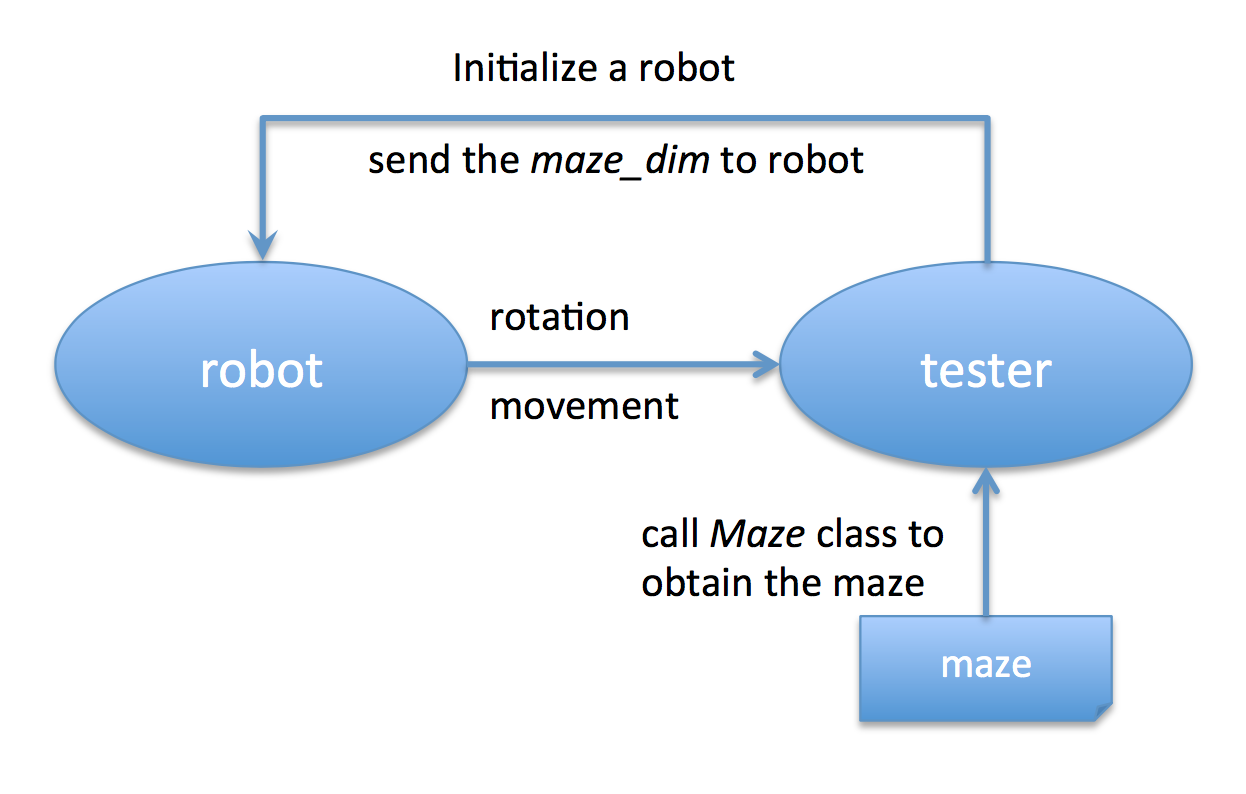
\includegraphics[width=14cm]{api.png} 
   \caption{The architecture of the robot and the test environment.}
   \label{fig:api} 
\end{figure}

For the purpose of clarity, I summarize some of the characteristics of the robot as below.
\begin{itemize}
\item The robot is always initialized by the tester. While the robot is initialized, its location is $(0,0)$ and heading is `up'.
\item The robot does not know any information about the given maze except the dimension. Of course, the maze is always a square.
\item The robot has to maintain the map of the maze when it visiting the maze.
\item The robot has three sensors mounted on the front of the robot, its right side, and its left side. These sensors can detect the distances from the robot to walls.
\item I implemented only one method (function), \texttt{next\_move}, for the \texttt{Robot} class. (Except the constructor, of course.)
\item The \texttt{next\_move} function must then return two values indicating the robot's rotation and movement on that time-step. Rotation is expected to be an integer taking one of three values: $-90$, $90$, or $0$, indicating a counterclockwise, clockwise, or no rotation, respectively. Movement follows rotation, and is expected to be an integer in the range $[-3, 3]$ inclusive.
\item The robot will attempt to move that many squares forward (positive) or backwards (negative), stopping movement if it encounters a wall.
\end{itemize}

The search algorithms implemented for the robot are DFS and A-star. In some sense, my DFS could be viewed as an A-star using heuristic matrix with $0$ in each entry. For an A-star search, the heuristic matrix plays a very important role in getting a good performance. I particularly mention my design of the heuristic matrix here.

For a $n\times n$ maze, my heuristic matrix, $H(i,j)$, is defined as below:


\begin{align*}
H(i,j)={\rm min}(\lVert (i,j)&-(\frac{n}{2}-1,\frac{n}{2}-1)\rVert , \\
\lVert (i,j)&-(\frac{n}{2}-1,\frac{n}{2})\rVert , \\
\lVert (i,j)&-(\frac{n}{2},\frac{n}{2}-1)\rVert , \\
\lVert (i,j)&-(\frac{n}{2},\frac{n}{2})\rVert ), 
\end{align*}
where $\lVert \cdot \rVert$ is 1-norm, which is defined as:
\[
\lVert {\bf v} \rVert = \sum\limits_{i=0}^k  \left| v_i\right|, 
\] 
where ${\bf v}=(v_0,v_1,v_2,\ldots ,v_k)$.

In particular, the heuristic matrix for $12\times 12$ maze is defined as:
$$\left[\begin{array}{cccccccccccc}
$10$ & $9$ & $8$ & $7$ & $6$ & $5$  & $5$ & $6$  & $7$  & $8$  & $9$  & $10$ \\
9&8  &7  &6  &5  &4  &4  &5  &6  &7  &8  &9 \\ 
  8& 7 &6  &5  &4  &3  &3  &4  &5  &6  &7  &8 \\ 
  7& 6 &5  &4  &3  &2  &2  &3  & 4 & 5 &6  &7 \\ 
   6& 5 &4  &3  &2  &1  &1  &2  & 3 &4  &5  &6 \\ 
 5& 4 & 3 &2  &1  &0  &0  &1  &2  &3  &4  &5 \\ 
5& 4 & 3 &2  &1  &0  &0  &1  &2  &3  &4  &5 \\ 
 6& 5 &4  &3  &2  &1  &1  &2  & 3 &4  &5  &6 \\  
 7& 6 &5  &4  &3  &2  &2  &3  & 4 & 5 &6  &7 \\  
 8& 7 &6  &5  &4  &3  &3  &4  &5  &6  &7  &8 \\ 
 9&8  &7  &6  &5  &4  &4  &5  &6  &7  &8  &9 \\ 
 10 & 9 & 8 & 7 & 6 &5  &5 &6  &7  &8  &9  &10  
\end{array}\right]$$

Now, we apply the heuristic matrix to the three given mazes, a preliminary result could be obtained. The following is the result while Maze01 is tested.
\begin{verbatim}
*******************************************************************************
Starting run 0.
[(0, 0), 'up'],
[(0, 1), 'up'],
[(0, 2), 'up'],
[(0, 3), 'up'],
[(0, 4), 'up'],
[(0, 5), 'up'],
[(0, 6), 'right'],
[(1, 6), 'right'],
[(2, 6), 'down'],
[(2, 5), 'right'],
[(3, 5), 'up'],
[(3, 6), 'up'],
[(3, 7), 'left'],
[(2, 7), 'left'],
[(3, 7), 'up'],
[(3, 7), 'up'],
[(3, 6), 'up'],
[(3, 6), 'up'],
[(3, 5), 'right'],
[(3, 5), 'down'],
[(3, 4), 'right'],
[(4, 4), 'up'],
[(4, 5), 'up'],
[(4, 6), 'up'],
[(4, 7), 'right'],
[(5, 7), 'right'],
[(6, 7), 'up'],
[(6, 8), 'left'],
[(5, 8), 'left'],
[(4, 8), 'up'],
[(4, 9), 'up'],
[(4, 8), 'left'],
[(4, 8), 'left'],
[(5, 8), 'left'],
[(5, 8), 'up'],
[(5, 9), 'right'],
[(6, 9), 'up'],
[(6, 10), 'left'],
[(5, 10), 'left'],
[(4, 10), 'left'],
[(3, 10), 'down'],
[(3, 9), 'down'],
[(3, 8), 'left'],
[(2, 8), 'up'],
[(2, 9), 'up'],
[(2, 10), 'left'],
[(1, 10), 'down'],
[(1, 9), 'down'],
[(1, 8), 'left'],
[(0, 8), 'down'],
[(0, 7), 'down'],
[(0, 8), 'left'],
[(0, 8), 'up'],
[(0, 9), 'up'],
[(0, 10), 'up'],
[(0, 11), 'right'],
[(1, 11), 'right'],
[(0, 11), 'up'],
[(0, 11), 'up'],
[(0, 10), 'up'],
[(0, 10), 'up'],
[(0, 9), 'up'],
[(0, 9), 'up'],
[(0, 8), 'left'],
[(0, 8), 'left'],
[(1, 8), 'down'],
[(1, 8), 'down'],
[(1, 9), 'down'],
[(1, 9), 'down'],
[(1, 10), 'left'],
[(1, 10), 'left'],
[(2, 10), 'up'],
[(2, 10), 'up'],
[(2, 11), 'up'],
[(2, 10), 'up'],
[(2, 10), 'up'],
[(2, 9), 'up'],
[(2, 9), 'up'],
[(2, 8), 'left'],
[(2, 8), 'left'],
[(3, 8), 'down'],
[(3, 8), 'down'],
[(3, 9), 'down'],
[(3, 9), 'down'],
[(3, 10), 'left'],
[(3, 10), 'up'],
[(3, 11), 'right'],
[(4, 11), 'right'],
[(5, 11), 'right'],
[(6, 11), 'right'],
[(7, 11), 'down'],
[(7, 10), 'right'],
[(8, 10), 'down'],
[(8, 9), 'left'],
[(7, 9), 'down'],
[(7, 8), 'down'],
[(7, 9), 'left'],
[(7, 9), 'left'],
[(8, 9), 'down'],
[(8, 9), 'down'],
[(8, 10), 'right'],
[(8, 10), 'right'],
[(9, 10), 'down'],
[(9, 9), 'down'],
[(9, 8), 'left'],
[(8, 8), 'down'],
[(8, 7), 'left'],
[(7, 7), 'down'],
[(7, 6), 'left'],
[(6, 6), 'up'],
Ending first run. Starting next run.
Starting run 1.
[(0, 0), 'up'],
[(0, 3), 'up'],
[(0, 6), 'right'],
[(2, 6), 'down'],
[(2, 5), 'right'],
[(3, 5), 'down'],
[(3, 4), 'right'],
[(4, 4), 'up'],
[(4, 7), 'right'],
[(6, 7), 'up'],
[(6, 8), 'left'],
[(5, 8), 'up'],
[(5, 9), 'right'],
[(6, 9), 'up'],
[(6, 10), 'left'],
[(3, 10), 'up'],
[(3, 11), 'right'],
[(6, 11), 'right'],
[(7, 11), 'down'],
[(7, 10), 'right'],
[(9, 10), 'down'],
[(9, 8), 'left'],
[(8, 8), 'down'],
[(8, 7), 'left'],
[(7, 7), 'down'],
[(7, 6), 'left'],
Goal found; run 1 completed!
Task complete! Score: 29.667
*******************************************************************************
\end{verbatim}

I plot the path on the maze. Figure x is the test result of Maze\_01; Figure x is the test result of Maze\_02; and Figure x is the test result of Maze\_03. 




\subsection{Refinement}




%%%%%%%%%%%%%%%%%%%%%%%%%%%%%%%%%%%%%%%%%%%%%%%%%%%%%%%%%%%%%%%%%%%%%%%%%%%%%%%%%%%
\section{Results}
This section includes two subsections: {\it Model Evaluation and Validation} and {\it Justification}.
\subsection{Model Evaluation and Validation}
\subsection{Justification}


%%%%%%%%%%%%%%%%%%%%%%%%%%%%%%%%%%%%%%%%%%%%%%%%%%%%%%%%%%%%%%%%%%%%%%%%%%%%%%%%%%%
\section{Conclusions}
Three subsections are included in this section. They are: {\it Free-Form Visualization}, {\it Reflection}, and {\it Improvement}.
\subsection{Free-Form Visualization}
(Use this section to come up with your own maze. Your maze should have the same dimensions (12x12, 14x14, or 16x16) and have the goal and starting positions in the same locations as the three example mazes (you can use test\_maze\_01.txt as a template). Try to make a design that you feel may either reflect the robustness of your robot's algorithm, or amplify a potential issue with the approach you used in your robot implementation. Provide a small discussion of the maze as well.)
\subsection{Reflection}
\subsection{Improvement}
(Consider if the scenario took place in a continuous domain. For example, each square has a unit length, walls are 0.1 units thick, and the robot is a circle of diameter 0.4 units. What modifications might be necessary to your robot’s code to handle the added complexity? Are there types of mazes in the continuous domain that could not be solved in the discrete domain? If you have ideas for other extensions to the current project, describe and discuss them here.)

\begin{thebibliography}{1}

  \bibitem{apec} {\em APEC Micromouse Contest Rules 2015}, http://www.apec-conf.org/wp-content/uploads/2013/10/APEC\_2015\_Micromouse\_Contest\_Rules.pdf

  \bibitem{Eranki} Rajiv Eranki, {\em Pathfinding using A* (A-Star)}, http://web.mit.edu/eranki/www/tutorials/search/, 2002. 

  \bibitem{G5AIAI} {\em G5AIAI-- Introduction to Artificial Intelligence: Blind Searches}, http://www.cs.nott.ac.uk/~pszgxk/courses/g5aiai/003blindsearches/blind\_searches.htm

  \bibitem{Nilsson} Nils J. Nilsson, {\em Artificial Intelligence: A New Synthesis}, 1st edition, Morgan Kaufmann Publishers, Inc., 1998.

  \bibitem{Russell-Norvig} S. Russell and P. Norvig, {\em Artificial Intelligence: a modern approach}, 3rd edition, Pearson Education, Inc., publishing as Prentice Hall, 2010.


  \bibitem{Shibuya} Naoki Shibuya, ``Plot and Navigate a Virtual Maze'', {\em Udacity Machine Learning Nanodegree Capstone Project Sample Report}, https://github.com/udacity/machine-learning/blob/master/projects/capstone/report-example-3.pdf, March 20, 2016.

  \bibitem{wikidfs} Wikipedia, {\em Depth-first search,} https://en.wikipedia.org/wiki/Depth-first\_search

  \end{thebibliography}

\end{document}  